\documentclass{llncs2e/llncs}

\usepackage{verbatim}
\usepackage[utf8]{inputenc}
\usepackage{graphicx}
\usepackage{bibentry}
\usepackage[numbers]{natbib}
\usepackage{fancyvrb}
\usepackage{epstopdf}

\title{An Argumentative Approach for a BDI Agent} 
        
\author{I\~{n}aki Garay \and      % igarai@gmail.com
        Diego Marcovecchio \and   % diegomarcov@gmail.com
        Leonardo Molas \and       % leos.molas@gmail.com
        Emiliano Montenegro \and  % emm.montenegro@gmail.com
        Fernando Sisul \and       % fsisul@gmail.com
        Manuel Torres \and        % jmtorresluc@gmail.com
        Sebastián Gottifredi \and % sebastian.gottifredi@gmail.com
        Alejandro García \and     % ajg@cs.uns.edu.ar
        Diego Martínez \and       % dcm@cs.uns.edu.ar
        Guillermo Simari          % grs@cs.uns.edu.ar
        }

\institute{Universidad Nacional del Sur \\\email{\{igarai,diegomarcov,leos.molas,%
emm.montenegro,fsisul,jmtorresluc\}@gmail.com,\\\{sg,ajg,dcm,grs\}%
@cs.uns.edu.ar}}

\begin{document}

\maketitle

\begin{abstract}
    This report presents the design and results of the d3lp0r multi-agent system 
    developed by the LIDIA team for the Multi-Agent Programming Contest 2011 (MAPC).
    The d3lp0r agents use a BDI architecture extended with planning and 
    argumentation (via Defeasible Logic Programming) to model a cooperating team 
    operating in a dynamic and competitive environment.

    In particular, the main goal of this report is to describe the chosen 
    architecture, the communication scheme and the way argumentation was put to 
    use in the agent's reasoning process and the technical details thereof.
\end{abstract}

\section{Introduction}

    The \texttt{d3lp0r} system was developed in the context of the Multi-Agent
    Programming Contest 2011 (MAPC) \cite{BehrensAMAI2010b} hosted by the
    Clausthal University of Technology \footnote{More information in
    \texttt{www.tu-clausthal.de}}.

    The LIDIA (Laboratorio de Investigación y Desarrollo en Inteligencia
    Artificial, Artificial Intelligence Research and Development Laboratory)
    research group was established in 1992 at the Universidad Nacional del Sur.
    The d3lp0r team was formed incorporating six graduate students, two Ph.D.
    students and three professors. The undergraduate students fully developed
    the system, while the Ph.D. students and professors provided guidance. The
    group's main motivation was to apply argumentation \cite{Prakken:1997}
    \cite{Rahwan:2009} \cite{Bench-Capon:2007}\ via defeasible logic programming
    (DeLP \cite{Garcia:2004a}) in a BDI based agent \cite{Amgoud:2008}, in the
    context of a multi-agent gaming situation, and to test the integration of
    the different technologies used.

%{{{
%\section{Preliminaries}
%
%    The \texttt{d3lp0r} system was developed in the context of the Multi-Agent
%    Programming Contest 2011 (MAPC) hosted by the Clausthal University of
%    Technology (www.tu-clausthal.de). 

%    The simulation scenario is represented as an undirected graph, in which 
%    nodes are valid agent locations weighted by value, and edges are valid
%    transitions weighted by cost. 
%    Agent state includes energy, health, and strength parameters. Agent percepts
%    include visible nodes, edges, and other agents. 
%    Each agent is assigned a role in the simulation (Explorer, Saboteur,
%    Repairer, Sentinel and Inspector) which determines its valid actions and
%    initial maximum values for the agent state parameters. 
%    Actions in general have an energy cost, movement action costs depend on edge
%    weights, successful attack actions decrease enemy agent's health subject to
%    a comparison of their strength attributes. Certain actions may cause further
%    information to be included in subsequent percepts. 
%
%    A match consists of several simulations, and each simulation proceeds as
%    a series of steps. In each step, each agent is provided with a percept with
%    partial information about the current simulation state and is
%    queried for its action. 
%
%    The goal is to maximize the score function each step. A team is awarded
%    points according to the value of the nodes controlled by the team, and
%    in addition certain achievements. Agents may control more nodes than 
%    those they are positioned in by forming zones, groups of nodes under the
%    influence of a team determined by a graph coloring algorithm specified in
%    the scenario description. 
%
%    The final score for a team is the sum of points over all steps; at the end
%    of the match, the team with the most points is the winner.
%}}}

\section{System Analysis and Design}

% 2 System Analysis and Design
% [x] 1. If some multi-agent system methodology such as Prometheus, O-MaSE, or
%        Tropos was used, how did you use it? If you did not what were the
%        reasons?
% [x] 2. Is the solution based on the centralisation of coordination/information 
%        on a specific agent? Conversely if you plan a decentralised solution, 
%        which strategy do you plan to use?
% [x] 3. What is the communication strategy and how complex is it?
% [x] 4. How are the following agent features considered/implemented: autonomy, 
%        proactiveness, reactiveness?
% [x] 5. Is the team a truly multi-agent system or rather a centralised system 
%        in disguise?
% [x] 6. How much time (man hours) have you invested (approximately) for 
%        implementing your team?
% [x] 7. Did you discuss the design and strategies of your agent team with other 
%        developers? To which extent did your test your agents playing with 
%        other teams?

    Despite many man-hours dedicated to design in the early stages of the
    competition, the development team's lack of experience in multi-agent
    systems made several changes and additions necessary and precluded the use
    of design methodologies specific to multi-agent systems.  The implementation
    was conducted using a simplified XP (extreme programming) methodology.
    [REFERENCIA] Nevertheless, our approach was more than satisfying, resulting
    to be modular, correct and in close correspondence with the literature.

    The solution follows a decentralised architecture in which agents run
    completely decoupled in different processes with no shared state. 
    
    % COMMUNICATION STRATEGY
    In addition to the agent processes, the system design includes an
    independent ``percept server'', through which percepts are communicated
    among agent team members via a broadcast mechanism running on standard
    network sockets.  Each agent handles his own connection to the MASSim
    server, and upon receiving its percept, retransmits it to the percept
    server.  The percept server joins all percepts into a ``global percept'',
    and sends each agent the set difference between its own and the global
    percept.  The agent then enters its reasoning phase and decides which
    action it will send back to the MASSim server.  Other than the percept
    server mechanism, there is no communication among team agents. This design
    was chosen for its minimal complexity.

    Agents can also be configured to run in a standalone mode, in which they will
    not use the percept server and thus have no communication with the rest of
    the team.  Team performance drops noticeably in this case, as the actions
    are less informed. 

    % DECENTRALISED, AUTONOMY
    Agents are completely autonomous meaning that decision-making takes place
    individually at the agent level, with no intervention from human operators
    or a central intelligence agency within the system, and that decisions made
    by an agent are influenced solely by the current simulation state and the
    results of previous steps.  
    Despite the sharing of all percepts among the team agents in the initial
    phase of the turn, no control variables or instructions are included. 
    The agent architecture developed is based on the
    BDI model \cite{Rao:1991}, and is explained in detail in further sections.

    The agents' behaviour can be considered proactive, given they pursue their 
    selected intentions over time, that is, they have persistent goals. Plans 
    for achieving intentions are recalculated and followed for the number of
    steps requiered, unless the goal in question becomes impossible or no longer
    relevant.

    Approximately 1500 man-hours were invested in the team development.

    Experience from a previous instance of the MAPC was shared with our teams by
    members of the ARGONAUTS team from TU Dortmund\cite{Holzgen:2011}. Although
    the initial plan was to run tests against other agent teams prior to the
    competition, time constraints made this impossible.


\section{Software Architecture}

%{{{
% SECTION: PROGRAMMING LANGUAGES; PLATFORMS AND TOOLS
% [x]  1. Which programming language did you use to implement the multi-agent 
%         system?
% [x]  2. Did you use multi-agent programming languages? Why or why not to use a 
%         multi-agent programming language?
% [ ] Question 3.2 not properly answered. General lack of flexibility: Why? Which languages did you use? Citation?
%    3.2: Did you use multi-agent programming languages? Why or why not to use a multi-agent programming language?

% [x]  4. Which development platforms and tools are used? How much time did you 
%         invest in learning those?
% [x] Question 3.4 not properly answered. Question was more about the question
% what editor did you use for the design process what IDE did you use, what
% about debugger for DeLP, etc. And the hours spent to learn how to use them.
%    3.4: 4. Which development platforms and tools are used? How much time did you invest in learning those?
%            editor for the design process? 
%            what IDE did you use?
%            what abpout debugger for delp?
%            hours spent learning those?
%
%        poner que no usamos IDEs 
%        poner lo del visualizador del arboles dialecticos de delp?

% [x]  5. Which runtime platforms and tools (e.g. Jade, AgentScape, simply Java, 
%         ....) are used? How much time did you invest in learning those?
% [ ]  6. What features were missing in your language choice that would have 
%         facilitated your development task?
% [x]  7. What features of your programming language has simplified your 
%         development task?

% SECTION IMPLEMENTION
% [x]  3. How have you mapped the designed architecture (both multi-agent and 
%         individual agent architectures) to programming codes, i.e., how did 
%         you implement specific agent-oriented concepts and designed artifacts 
%         using the programming language?

% [ ] 10. To which extent is the reasoning of your agents synchronized with the 
%         receive-percepts/send-action cycle?
% [ ] Question 3.10 is not discussed in the paper. Do you do reasoning between two steps?

% [ ] How does the static, dynamic and initial data look like?
% [x] How does DeLP look like? Only explained later.
% [ ] How does an intention look like?

% [x]  8. Which algorithms are used/implemented?

% [x]  9. How did you distribute the agents on several machines? And if you did 
%         not please justify why.

% SECTION: DIFFICULTIES ENCOUNTERED
% [ ] 11. What part of the development was most difficult/complex? What kind of 
%         problems have you found and how are they solved?

% [x] 12. How many lines of code did you write for your software?
% [x] Question 3.12 not answered.

% This section is a little bit unsorted and too short. I think you should first
% explain the overall structure, then describe each node in detail, i.e., parts
% from 4.2 should go to 4.1.
% Without looking into the source code the reader cannot understand how the agent
% team works, e.g., how do the agents synchronize their intentions?
% In general, a lot of information is missing in order to understand the ideas
% behind the agent team. How do you deal with updates that invalidates old
% information? What about an example? What does the belief base contain? only
% percepts?
% 
%    IÑAKI:
%        como se representa el conocimiento?
%        how does de static dynamic and initial data look like?
%        como se representa entre el agente y el PS?
%        ejemplos de codigo 
%        como se traduce a prolog para meterlo en la KB?
%        UNA BUENA EXPLICACION DEL PIPELINE DE DATOS
%    MANU: how does an intention look like?
%
%    cada turno la informacion en la kb se actualiza, se usa el parametro de step para ver la edad y validez de la info
%    ejemplo el algoritmo de coloreo permite generacion de creencias, por lo cual en la kb no esta solamente la percepcion
%}}}

\subsection{Programming languages, platforms and tools}
    %{{{
    The agent system was implemented using Python 2.7 and SWI Prolog
    5.10.5.  Language integration was achieved using the \textit{pyswip}\
    library\footnote{http://code.google.com/p/pyswip/}, which facilitates the
    execution of Prolog queries from Python.  The implementation of Defeasible
    Logic Programming (DeLP) by the LIDIA \cite{Garcia:2004a} was used for the
    deliberative process, in which desires and intentions are set.  The
    standard Python and SWI-Prolog debugging tools were used.  DeLP includes
    a graphical viewer for dialectical trees, allowing visualization of which
    arguments attack others and facilitating debugging of the defeasible rules
    employed.  These languages and platforms were well-known at the start of
    the project, and were chosen for precisely those reasons.
    
    No multi-agent programming languages / platforms / frameworks were used due to 
    a lack of familiarity on behalf of the development team. 
    Also, integrating or extending an existing framework with queries to
    defeasible rules was initially considered more difficult than the
    straighforward approach taken.

    Python's amenity to rapid application development and ``batteries-included 
    philosophy'' facilitated implementing the communication layer to the MASSim 
    server, parsing of perceptions, rapid addition of planned features and bug 
    correction. DeLP's capability to deal with conflicting pieces of
    information was also very helpful in order to implement the
    decision-making module. 
    %}}}

\subsection{Implementation}
    %{{{
    The system was implemented as a collection of independent operating system
    processes, the percept server (PS from here onwards) and each agent running
    in its own address space.  The agents are started individually and
    synchronize via the PS.  Each one handles its own connection to
    the MASSim and percep servers, as the \textit{eismassim} package provided
    by the contest organizers was not used to avoid the difficulty of
    integrating yet another language and runtime (Java) with the ones being
    used. 
    
    \begin{figure}
    \centering
    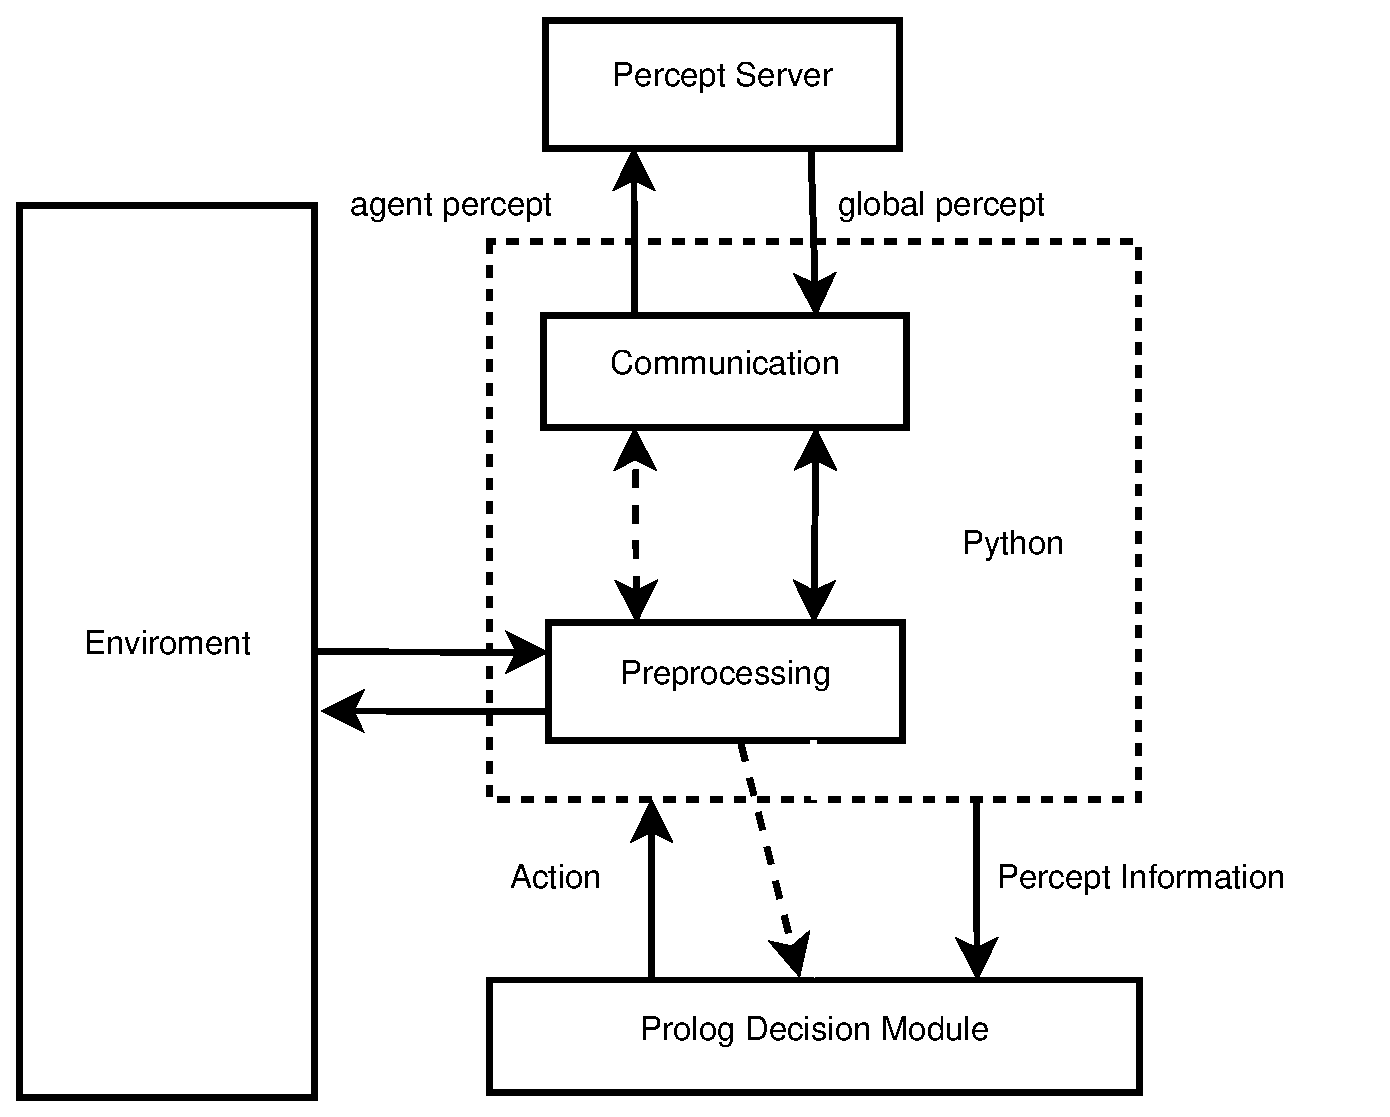
\includegraphics[scale=.3]{agentarchitecture.eps}
    \caption{Agent architecture in a flow chart-like diagram. Dashed arrows
    represent process flow, solid lines represent data flow.}
    \label{fig:architecture}
    \end{figure}

    \begin{figure}[!htb]
    \centering
    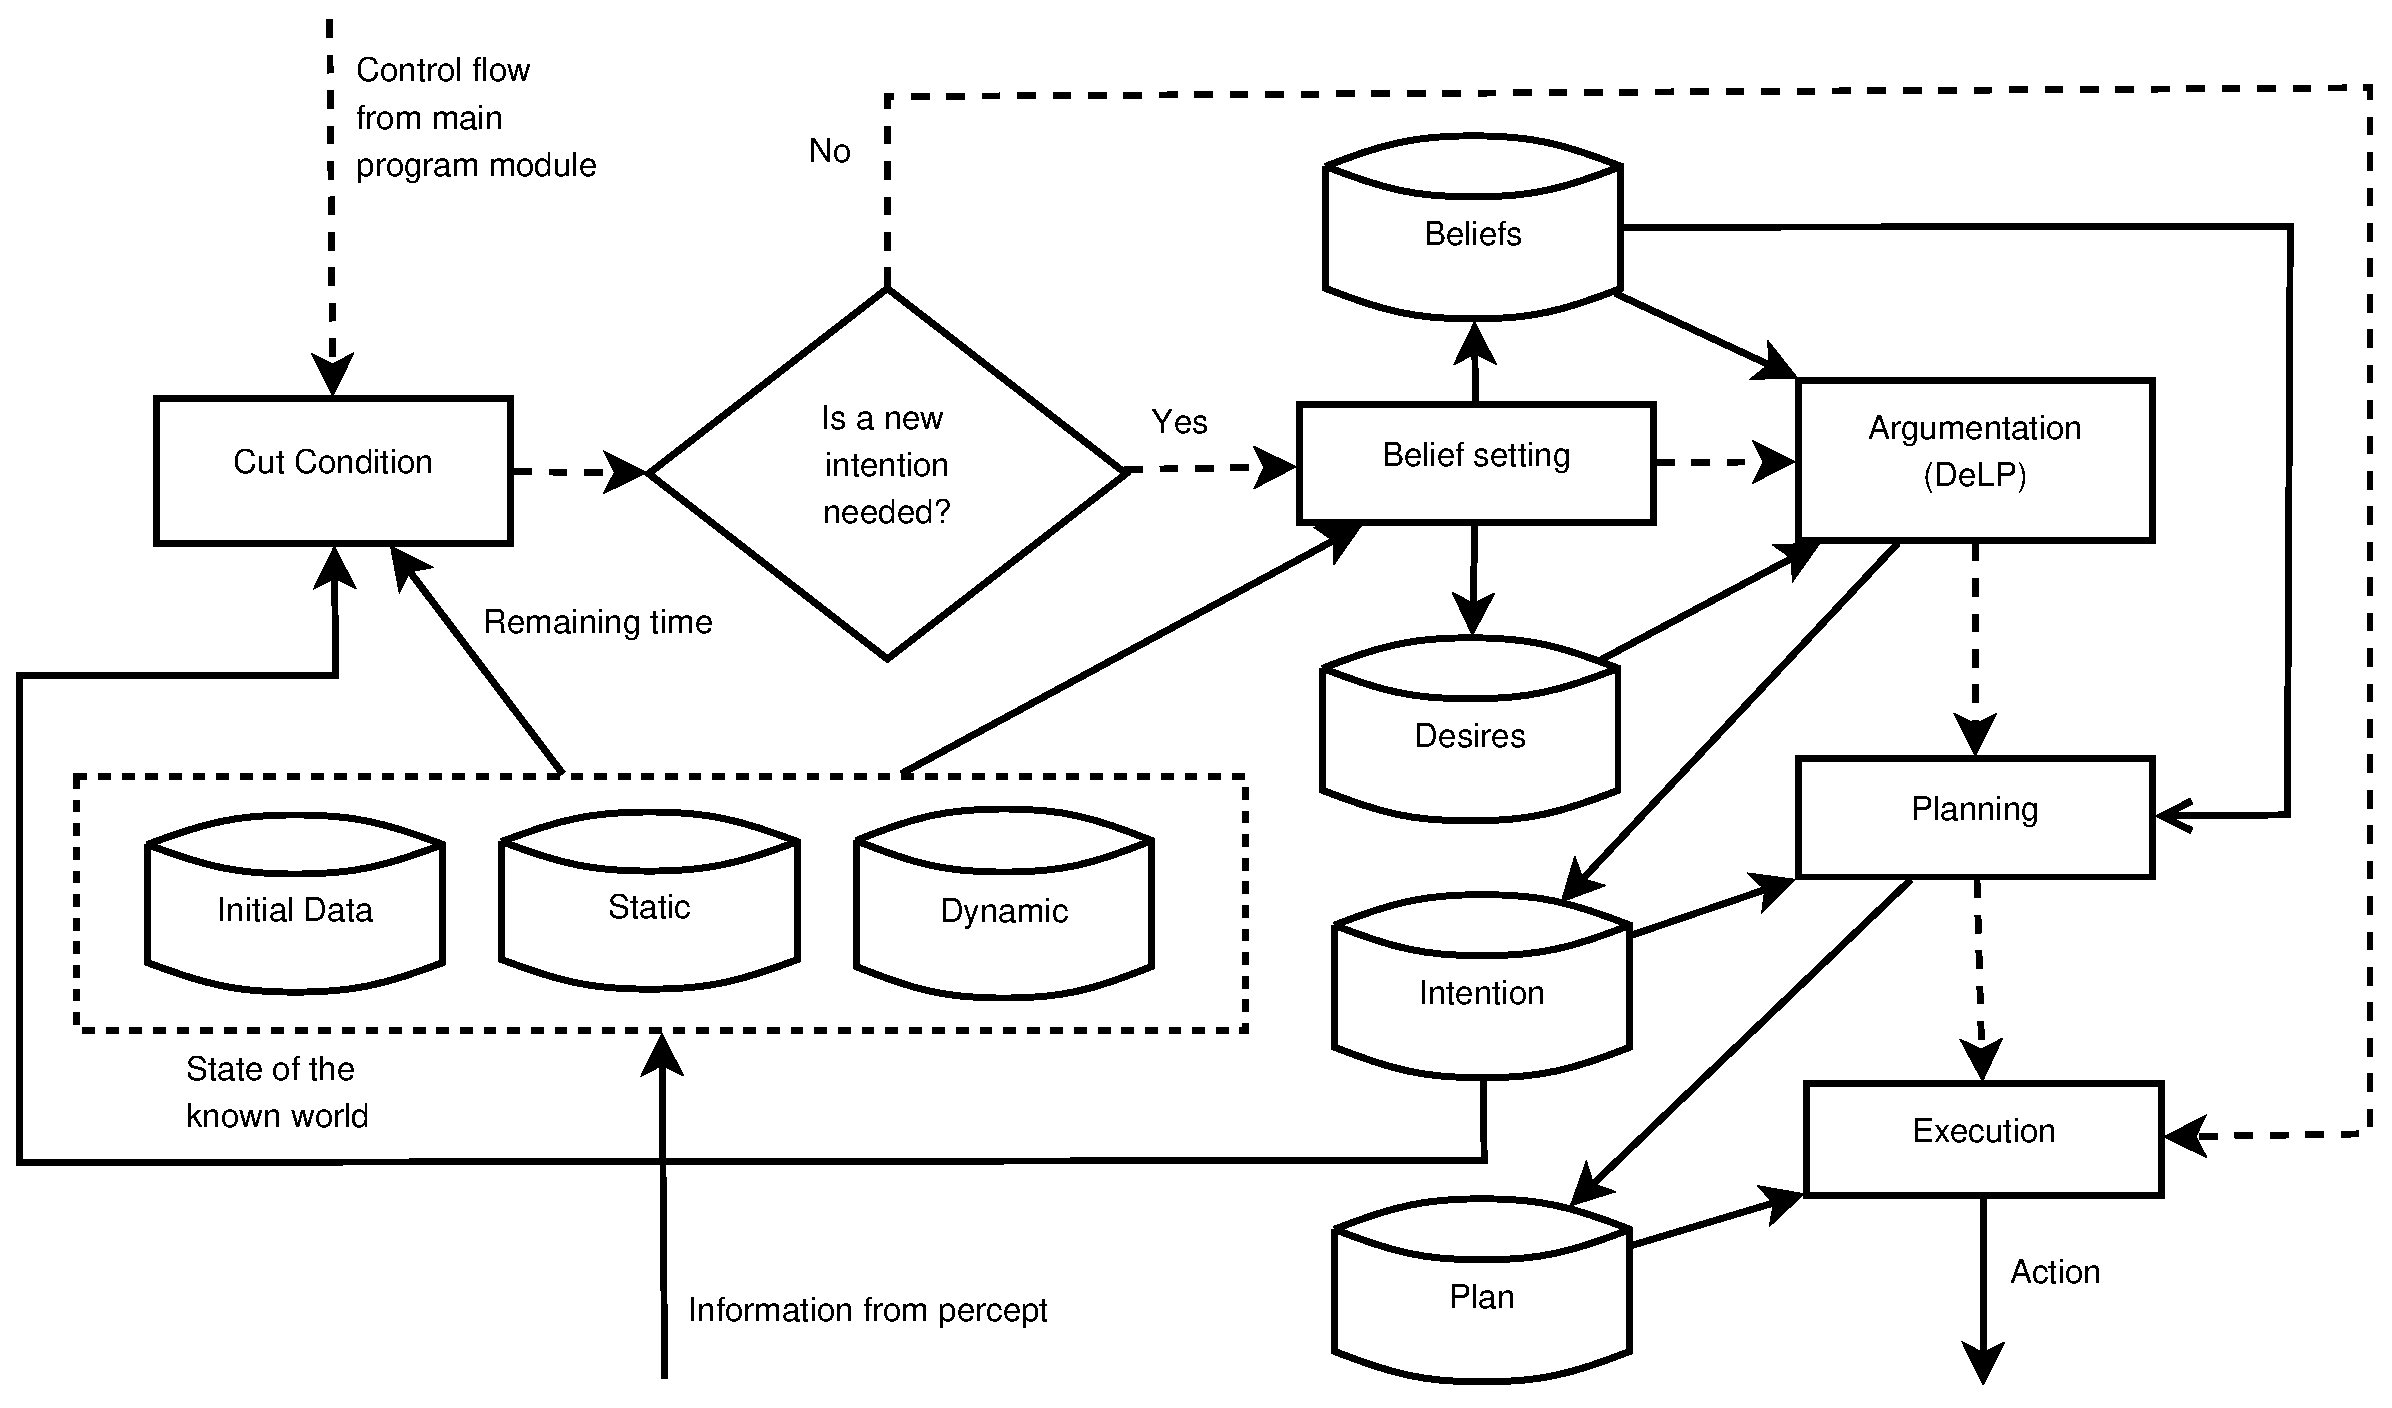
\includegraphics[width=\textwidth]{agentprolog.eps}
    \caption{Architecture of the Prolog decision module}
    \label{fig:prologmodule}
    \end{figure}

    Fig. \ref{fig:prologmodule} shows the structure and flow of control and
    information within the decision making module implemented in Prolog and
    DeLP.
    %}}}
    
\subsubsection{Agent main program.}
    %{{{
    The agent main program is implemented in Python, and handles all
    communication with the servers, XML parsing, processing the information in
    the percept into a form suitable for assertion in the agent's knowledge
    base, and generation of the XML representing the action taken which is
    returned to the MASSim server.

    Initialization consists of opening the connections to the MASSim server,
    authenticating, opening the connection to the PS, and starting
    the Prolog engine. The main program loop is then entered, in which messages
    from the MASSim server are received and parsed. 

    When a message of type \texttt{sim-start} is received, initial information
    present in the message such as the agent's role and the simulation
    parameters are asserted into the agent's knowledge base and the perceive-act
    loop is started.

    Each iteration of the perceive-act loop expects a \texttt{request-action}
    message from the MASSim server and parses the XML into a Python dictionary.
    Elements in the percept are divided into a ``public'' section, which is sent
    to the PS to be shared with other team agents and a ``private''
    section.

    The agent will then send the percept to the PS and await the global percept
    containing the remainig information perceived by the team. The global
    percept is merged with it's own, and asserted into the agent's knowledge
    base, establishing the agent's beliefs.  Note that no information is
    included in the percept other than what is received in the percept.

    The decision making module implemented in Prolog is then queried for the
    next action to be performed by the agent.  Once control flow returns to the
    Python program with the determined action, the corresponding XML message is
    generated and sent to the MASSim server. 
    %}}}

\subsubsection{Percept Server.}
    %{{{
    The PS maintains a connection for each agent.  The connection handling
    methods encode the associate array into a form suitable for conversion into
    a set datastructure, which is then sent over the network.  On each
    iteration, the PS waits for each agent's data, performs a union of all data
    sets, and returns to each agent the set difference between the data the
    agent sent and the total union.  Figures \ref{fig:pythonperceptpublic} and
    \ref{fig:pythonperceptprivate} show example percepts after parsing, before
    being sent to the percept server.

    \begin{figure}
    \centering
    \label{fig:pythonperceptpublic}
    \begin{small}
    \begin{verbatim}
    { 'surveyed_edges' : [ ], 
      'vis_verts'      : [ { 'name': 'vertex65',  
                             'team': 'none' }, 
                           ...  ],  
      'vis_ents'       : [ { 'node':   'vertex97',  
                             'status': 'normal', 
                             'name':   'a6',  
                             'team':   'A' }, 
                             ...  ],  
      'inspected_ents' : [ ],  
      'vis_edges'      : [ { 'node1': 'vertex141', 
                             'node2': 'vertex65' }, 
                           ...  ], 
      'position'       : [ { 'node':       'vertex141', 
                             'vis_range':  '1', 
                             'health':     '6', 
                             'name':       'self', 
                             'max_health': '6' } ], 
      'probed_verts'   : [ ] }
    \end{verbatim}
    \end{small}
    \caption{A sample public section of a percept, after parsing.}
    \end{figure}

    \begin{figure}
    \centering
    \label{fig:pythonperceptprivate}
    \begin{small}
    \begin{verbatim}
    { 'total_time':      2000L, 'zone_score': '0',            
      'last_step_score': '20',  'timestamp':  '1323732915832',       
      'strength':        '0',   'energy':     '11',                  
      'money':           '12',  'max_energy_disabled': '16',                  
      'last_action':     'recharge', 'max_health':     '6',
      ... }
    \end{verbatim}
    \end{small}
    \caption{A sample private section of a percept.}
    \end{figure}
    %}}}

\subsubsection{Beliefs-Desires-Intentions}
    %{{{
    Once the remaining information is received from the percept server, the data
    is then asserted into the agent's knowledge base. A collection of predicates
    queried from the main Python module are in charge of verifying that
    information is not overwritten, and that redundant information is not
    inserted. Most predicates which represent the state of the environment
    include a parameter bound to the turn the information was perceived, so that
    information can be considered ``stale'' if the difference between the
    current turn and the turn the information was acquired is too large.
    
    Beliefs in the knowledge base are represented as terms, arguments to the
    predicate \texttt{b/1}.  Desires are also represented as Prolog terms;
    possible desires are \texttt{expansion} (increase the value of a zone),
    \texttt{explore} (probe nodes and increase the team's knowledge of the
    graph), \texttt{regroup} (move closer to team members),
    \texttt{seekforrepair} (move closer to an agent with the \textit{repairer}
    role), \texttt{selfdefense}, \texttt{parry}, \texttt{stay} (do not move),
    \texttt{buy}, \texttt{probe}, \texttt{repair}, \texttt{attack}. The desires
    an agent may entertain depend on the agent's role. 
    
    The intention is selected from the set of possible desires the agent may
    entertain.  If the agent already has an intention stored, the \textit{cut
    condition} checks whether it makes sense to keep trying to fulfill it. It is
    a series of simple conditions that review the state of the world.

    Then, if there is not any commited intention, or the cut condition decides
    it is not interesting to keep it, the \textit{beliefs setting process} is
    started. It generates the possible desires for this step, according to what
    is stored in the knowledge base, and, for each one of them, the beliefs
    needed.  The decision-making module is implemented in
    DeLP \cite{Rotstein:2007} \cite{Ferretti:2008}, a defeasible logic
    programming language that uses argumentation \cite{DBLP:conf/comma/2008}\ to
    reason with conflicting information.  Given the set of possible desires and
    beliefs set by the previous module, it selects the best desire, returning it
    as the intention that the agent commits to achieve.

    All the plans for all the desires were previously calculated and stored as 
    beliefs, since the amount of steps that they take is used by the 
    argumentation module. The \textit{planning} module selects the one 
    corresponding to the selected intention, and stores it. Then, the 
    execution module only gets the plan, and returns to Python the first 
    action in it.
    For both search algorithms, the Depth First Search and the Uniform Cost 
    Search, we added conditions that could cut several branches, when they were 
    expanding to unwanted nodes. This conditions were set by the caller, since 
    they depend on the context of the problem.

    For the UCS, we first used a simple stack implemented with a list, to keep 
    track of the frontier, because of Prolog's inability to work with arrays. This 
    would have allowed us to develop a heap data structure, to be used in a 
    priority queue. Lately, we found a Prolog library that implemented this data 
    structure, and the migration was pleasantly straightforward.

    However, if the process flow comes from the other branch of Fig. 
    \ref{fig:architecture} (that is, after the cut condition, the agent has an 
    intention), the execution is not that simple. Since skipping the decision-
    taking makes this branch insignificant in terms of time, we decided to 
    recalculate the plan. This might help us when a better path is discovered, 
    even though this is unlikely.
    %}}}

\subsubsection{Deliberation and DeLP.}
    \newcommand{\drule}[2]{\mbox{$ #1\; \defleftarrow \; #2$}}
    \newcommand{\defleftarrow}{{\raise1.5pt\hbox{\tiny\defleft}}}
    \newcommand{\defleft}{\mbox{---\hspace{-1.5pt}\raise.05pt\hbox{$<$}}}
    %{{{
    In DeLP\cite{Garcia:2004a}, knowledge is represented using facts, strict rules
    and defeasible rules. Facts and strict rules are ground literals representing
    firm information that can not be challenged. \textit{Defeasible Rules}
    (d-rules) are denoted $\drule{L_0}{L_1, \ldots, L_n}$ (where $L_i$ are literals)
    and represent tentative information. These rules may be used if nothing could
    be posed against it. A d-rule \textit{``\drule{Head}{Body}''} expresses that
    \textit{``reasons to believe in Body give reasons to believe in Head''}. A DeLP
    program is a set of facts, strict rules and defeasible rules. 

    {\it Strong negation} is allowed in the head of program rules, and hence, may
    be used to represent contradictory knowledge. From such a program contradictory
    literals could be derived, however,  the set of facts and strict rules must
    possess certain internal coherence (it has to be non-contradictory). 

    To deal with contradictory information, in DeLP, \emph{arguments} for
    conflicting pieces of information are built and then compared to decide
    which one prevails. The prevailing argument is a \emph{warrant} for the
    information that it supports.  In DeLP, a query $L$ is \emph{warranted} from
    a program if a \emph{non-defeated} argument that supports $L$ exists. %\Arg\ 
    
    \begin{figure}
    \begin{small}
    \begin{Verbatim}
    selfDefense(1000) -<
        myStatus(normal), canParry,
        myPosition(Node), enemySaboteurPosition(Node).  

    canParry -< myRole(repairer).  canParry -< myRole(saboteur).
    canParry -< myRole(sentinel).  
    ~canParry <- myEnergy(Energy), less(Energy, 2). 
    \end{Verbatim}
    \end{small}
    \caption{Desire \texttt{SelfDefense}}
    \label{fig:SelfDefense}
    \end{figure}
    
    Figure \ref{fig:SelfDefense}\ is an example of our representation of the
    possible intentions written in DeLP.  Self defense has a weight of 1000. It
    is a high priority intention given that the average weight of the intentions
    is around 150.  \texttt{myStatus}, \texttt{myPosition},
    \texttt{enemySaboteurPosition}, \texttt{myRole} and \texttt{myEnergy} are
    facts of the knowledge base. \texttt{canParry} is an argument that supports
    or defeats the argument for the Self Defense intention.    
    canParry arguments will support or defeat arguments for selfdefense intention
    %}}}

\subsection{Difficulties encountered}
    %{{{
    The most difficult problems were related to optimization. Much of our time was 
    spent in reducing the complexity of our algorithms, and the times they 
    were called.

    Our initial plan was to distribute agents on several machines. Each agent runs 
    as a separate process, and communicates with others via TCP sockets. After 
    some experience and benchmarking, agents were run on one machine, due to 
    For both search algorithms, the Depth First Search and the Uniform Cost 
    Search, we added conditions that could cut several branches, when they were 
    expanding to unwanted nodes. This conditions were set by the caller, since 
    they depend on the context of the problem.

    For the UCS, we first used a simple stack implemented with a list, to keep 
    track of the frontier, because of Prolog's inability to work with arrays. This 
    would have allowed us to develop a heap data structure, to be used in a 
    priority queue. Lately, we found a Prolog library that implemented this data 
    structure, and the migration was pleasantly straightforward.

    performance issues. 
    Having the choice was a benefit of the proposed design.
    %}}}

In total, the system consists of 1336 lines of Python, 5059 lines of Prolog
pertaining strictly to the agent, belief setting and auxiliary predicates, and
355 lines of DeLP rules, both defeasible and strict.  The DeLP interpreter
consists of 4494 lines of Prolog. These figures includes commentaries and blank
lines. 

%Python:             1336
%Prolog:             5059
%Interprete DeLP:    4494
%DeLP:               355


\section{Strategies, Details, and Statistics}

% 4 Strategies, Details and Statistics
% [ ]  1. What is the main strategy of your team?
% [ ]  2. How does the overall team work together? (coordination, information sharing, ...)
% [ ]  3. How do your agents analyze the topology of the map? And how do they exploit their findings?
% [ ]  4. How do your agents communicate with the server?
% [ ]  5. How do you implement the roles of the agents? Which strategies do the different roles implement?
% [ ]  6. How do you find good zones? How do you estimate the value of zones?
% [ ]  7. How do you conquer zones? How do you defend zones if attacked? Do you attack zones?
% [ ]  8. Can your agents change their behavior during runtime? If so, what triggers the changes?
% [ ]  9. What algorithm(s) do you use for agent path planning?
% [ ] 10. How do you make use of the buying-mechanism?
% [ ] 11. How important are achievements for your overall strategy?
% [ ] 12. Do your agents have an explicit mental state?
% [ ] 13. How do your agents communicate? And what do they communicate?
% [ ] 14. How do you organize your agents? Do you use e.g. hierarchies? Is your organization implicit or explicit?
% [ ] 15. Is most of your agents’ behavior emergent on and individual and team level?
% [ ] 16. If your agents perform some planning, how many steps do they plan ahead?
    
    In this section, we will explain the main characteristics of the team's 
    overall strategy, as well as several implementation details, such as 
    algorithms used and agents' organization.

\subsection{Strategy}

    The main strategy of the team consists of detecting profitable zones from the 
    explored nodes, and positioning the agents correctly to maintain, defend 
    and expand the zones formed. 
    
    To accomplish this, all agents follow the same concept. Every agent is concerned 
    with the formation and expansion of zones, beyond its role.
    The desicion-taking process is responsible for calculating and selecting the
    most beneficial intention, which may be focused in the zone conquering (if possible),
    or not.
    This selection process is based on many factors, such as the gain in terms 
    of score, the need of the team for the execution of a role-specific action, or
    the benefit that the agent is currently contributing to the team. 
    
    For example, a repairer agent that is part of a zone will attempt to keep or
    expand the zone by moving to a better node (in terms of zone coloring), 
    unless a teammate needs to be repaired.
    
    Agents coordination is achived in an implicit way. This is, the information
    shared consists only of the perception received, not including neither 
    preprocessed beliefs, nor control variables. The agents do not communicate
    their intentions nor plans, so any coordination that they may exhibit is 
    accomplished implicitly.

    % TODO: revisar el inglés de esta oración. No nos convence el "or" de dos
    % lineas antes.
    % TODO revisar el doble uso de neither nor, juntar las oraciones?
       
\subsubsection{Zone conquering}
    
    The exploration of the map is done gradually, as a result of the reasoning 
    proccess. The actions related to the exploration (probe, survey) are weight 
    along with all other actions and are selected when it is considered important. 
    This is seen to a greater extent during the inicial steps of the simulations, 
    when the team lacks of knowledge about the map and other kind of actions are 
    unnecesary. Agents make no assumptions about the map topology.

    Agents are not primarily focused on finding new zones, but they attempt to 
    expand and maximize the points of the existing ones.    
    They calculate whether they are part of a zone or not. This is achieved
    by checking the color of the current node (received in the perception), and if
    a neighbor of it is also colored by the agent team (if this is not the case, the 
    node does not increase the zone points).
    If an agent is not being part of any zone, it tries to regroup with its 
    teammates. 

    When a zone is formed, and the agent is part of it, for each potentially 
    beneficial neighbor node, the agent calculates how much points would the team 
    gain if it moves, and tries to expand the zone.
    If the expansion intention explained is selected and carried on, then a new 
    better zone is implicitly conquered.
    
    This estimations are done with our reimplementation of the coloring algorithm used 
    by the MASSim server. The information is used by the decision taking module.  

\subsubsection{Attacking and defending}
    
    Both attacking and defense of zones are implicitly implemented. 
    Sabouteurs prefer to attack enemies that are near, so if an agent of another 
    team enters our team's zone, it will be attacked by the saboteurs in the zone.
    This is the most likely scenario, unless the saboteur's position is so 
    important that it decides to stay in the formation in order to keep the zone.

    The same happens with enemies in their own zones. Zones are not intentionally 
    destroyed, but any agent that is part of a zone may be attacked, affecting 
    posibbly the structure of the enemy zone.
    
    Agents of other roles can also implicitly defend a zone. For example, an agent 
    can go to a node that has one agent of each team, with the purpose of coloring the 
    contested node and defending the zone.
    
\subsubsection{Phases}

    Our agents do not change their behavior during runtime. This feature was 
    analysed, but the team did not have enough time to finish its implementation.
    
    The approach proposed consists in adding a phase indicator that holds different 
    phase values like 'exploration', or 'expansion'. The phase is updated at runtime
    considering elements like the number of steps or the team's overall performance 
    in the simulation in progress.
    
    The phase component is weight as an extra factor that modifies the potential 
    benefit of each action, so that its inclusion directly affects the action-selection 
    proccess.
    
\subsubsection{Buying}

    Agents follow a list of predefined buying actions, when the necessary amount 
    of money is reached. This behaviour follows the idea of getting some specific skill 
    upgrades that the team considered important to achieve early in the simulations.
    
    Many other approaches regarding the use of the earned money were considered as well.
    % No se si el regarding esta bien usado.
    For example a more thoughtful one, taking into consideration the amount of deaths 
    of our team and our enemy. However, this simple approach was the easiest to implement, 
    and it was proven to be the most succesful one.

\subsubsection{Achievements}

    Achievements are not explicitly taken under consideration. That is, the agents'
    reasoning proccess is not affected by the possibility of completing achievements.    
    However, the team can manage to achieve a significant number of them, which 
    results naturally from the agents' behaviour. 
    This fact let the development team avoid the need of adding special features 
    dedicated to the seek of achievements.
    
\subsection{Implementation}

    Here are some implementation details of the different parts of the agents.
    
\subsubsection{Mental state.}

    Agents have a complete and explicit mental state. It consists of a set of 
    components, such as beliefs, desires, intentions, and plans. 
    The belief base includes the information obtained from the perceptions, as
    well as different kinds of beliefs required by the decision-taking module.
    The desires are set every step that the agent decides to select a new intention.
    The intentions and plans kept in the knowledge base are those that the agent
    is currently carrying out.
    
\subsubsection{Path planning.}

    Path planning is implemented with an Uniform Cost Search 
    \cite{Russell:2003:AIM:773294}. 
    What we tried to minimize was the amount of steps required to achieve the 
    goal, rather than the energy spent. 
    The returned result is a list of actions to be done, rather than a list of 
    nodes.
    
    Since this algorithm can be called several times in one step, and given that the 
    actual amount of steps spent by an intention is taken under consideration by 
    the decision-taking module, it was crucial to perform several optimizations in 
    it. In the end, this allowed us to run all the agents in a single machine  
    during the competition.
    
    The plans are as long as the selected intention requieres. This may 
    sound excesive, but the possible goals were previously selected for their 
    potential, taking into consideration their distances (in nodes, not in 
    actions). However, plans are recalculated in every step, as explained earlier.    

\subsubsection{Communication.}

    Some functionality provided by the \textit{eismassim} library was
    reimplemented in a connection library in Python.

    On each perceive/act cycle, agents receive the percept from the MASSim server, 
    separate the information which will remain private and which will be shared. 
    The public part of the percept is sent to the percept server, which performs a 
    union of all percepts and send the difference back to each agent. After 
    receiving the joint percept, the agents enter a belief setting phase, and 
    later an argumentative phase.

\subsection{Agents' organization}

    As explained before, all agents operate in the same way. The desicion-taking
    module makes use of other agents' status, but there is neither negotiation nor 
    intentions exchange, so the team performance is emergent on an individual behaviour. 
    The only organization that they have is the proper given by the environment, 
    which is the roles.
    
    Refering to our actual programming, all the agents have a strong core of common
    code, which is:
    
    \begin{itemize}
    \item all the Python part, that servers as a receive-percepts/send-action client 
    of the server,
    
    \item the Percept Server,
    
    \item an important part of the Prolog code, including all the utilities used, the
    implementation of the BDI architecture, the structure of the 
    decision-taking module, and a considerable part of the arguments used, that
    are common to all the roles.
    \end{itemize}
    
    Apart from all this, each role has a couple of separate files, that have 
    specific code, including the arguments used in the decision-taking module, and
    the setting of the beliefs needed for those arguments. Here is where the 
    individual behavior is set, since the specific actions that can be done by each
    role are taken into consideration here.
    
    Specific values for the decision-taking module for each role are also included
    in these files, and this is what can make that agents of different roles act 
    differently faced to the same situation, according to our judgement.
    
    This separation is negligible, having in consideration the amount of code 
    written for the agents, and may be near a 5\% of it. However, this has been proven to
    be more than enough to modify considerably the behavior of the agents, thanks to
    the non-monotonic nature of DeLP, the argumentation language used in the 
    decision-taking module.

\section{Conclusion}

% 5 Conclusion
% [ ] 1. What have you learned from the participation in the contest?
% [ ] 2. Which are the strong and weak points of the team?
% [ ] 3. How suitable was the chosen programming language, methodology, tools, and algorithms?
% [ ] 4. What can be improved in the context for next year?
% [ ] 5. Why did your team perform as it did? Why did the other teams perform better/worse than you did?
% [ ] 6. Which other research fields might be interested in the Multi-Agent Programming Contest?
% [ ] 7. How can the current scenario be optimized? How would those optimization pay off?

\subsection{Our team, and its development}

    Our team is formed by a group of friends, so a strong point in the developing 
    process has been the cohesion and comradeship. We had also worked together,
    in university's projects as well as outside them, in small freelance 
    projects, so we well knew what to expect from each other, and each member's 
    capabilities. 

    Several events in the developing process depended on this bond, i.e. the 
    deployment. We could not connect to the server in the test matches from our 
    university, because of several network problems. Only one day before 
    the competition, we decided to connect everything from one of our partner's house, 
    who had the best infrastructure (connection to Internet, and space in his 
    apartment). Given the fact that we had to spend all night working and testing
    there, for a week the headquarters for our team also became our home.

    However, we had many problems. Many of them were related with our lack of 
    professionality, and lack of experience working in a large project. 
    For example, we had several simple but annoying problems, such as the 
    encoding of our source files, or having different versions of the programs 
    we used to program installed in our computers.

    We are really grateful with our decisions involving programming languages, 
    tools and algorithms. Of course, we had many problems, and much time was spent 
    deciding what to choose. Nevertheless, having all the process in 
    consideration, we may had took the right calls. We should thank the great 
    education given by our university (Universidad Nacional del Sur), and a 
    great mentoring from our professors.

    Many things should and will be improved for next year competence. We have
    gained an important amount of knowledge, capability and experience, that shall 
    help us in all aspects of the developing process, not to mention the 
    important amount of code already written, and all the good decisions already 
    made.

    In particular, we now know the importance of all the testing actually needed 
    for this sort of competition, not only in a virtual environment, as we did, 
    but also in the real context of the contest. There were several hotfixes that 
    were written and deployed at the same time we were facing our competitors, in 
    all but the last day of competition, in which we already had everything in 
    consideration and control.

\subsection{Our thoughts about possible optimizations to the contest}
    
    Many optimizations ocurred to us for the scenario, and the contest in general. 
    For example, more information for the nodes, including something useful for a 
    directed search (i.e., absolute coordinates), would help in the implementation 
    of an A* search, that would decrease the execution times.

    Strategically, the early dominion of the center area played an important part 
    of a good candidate to win a match. It would be useful to try other 
    variations, such as making the borders more important, or others shapes of the 
    map, such as stretched, in form of V, X, O, etc. This would benefit teams that 
    explicitly and thoughtfully look for and conquer good zones, rather than 
    benefiting teams that assume that only one good zone exists, and it's in the 
    middle of the map.

    More informing feedback from the server would be appreciated, specially
    involving errors. This is important for a better and quicker detection of bugs
    involving the communication, i.e. problems with the connection, files sent.

    Finally, we think it will be really helpful for all that we had test matches 
    in a more early stage, in order to have more time to correct errors in the 
    client. Many of us reimplemented the eismassim module, so we are vulnerable to 
    many errors that were difficult to foresee. Early testing would help with 
    that, and detecting infrastructure issues, such as network problems.
    
    % TODO pregunta 6 que otros campos
    % Game AI, Robotics

%BIBTEX
    
\bibliographystyle{plainnat} 
\bibliography{bib} 

%TL;DR section: (short answers for all questions)

\section{Short Answers}

% == Introduction 1. 

\subsection{Introduction}

\begin{question}
What was the motivation to participate in the contest?  
\end{question}

The group's main motivation was to apply argumentation via defeasible 
logic programming (DeLP) in a multi-agent gaming situation and to test the
integration of the different technologies used.

\begin{question}
What is the history of the team?  
\end{question}

The LIDIA research group was established in 1992 in the Universidad 
Nacional del Sur, and it is the first time our time participates in the 
contest.

\begin{question}
What is the name of your team?  
\end{question}

The team's name is d3lp0r.

\begin{question}
How many developers and designers did you have?  At what level of education
are your team members?  
\end{question}

The d3lp0r team was formed incorporating six graduate
students, two Ph.D. students and three professors.

\begin{question}
From which field of research do you come form?  Which work is related?  
\end{question}

The
LIDIA research group has been working in Artificial Intelligence and
Argumentation via Defeasible Logic Programming for almost 20 years now, and
the DeLP server technology developed has been used in the contest.

\subsection{System Analysis and Design}
\setcounter{question}{0}
% == System Analysis and Design
\begin{question}
If some multi-agent system methodology such
as Prometheus, O-MaSE, or Tropos was used, how did you use it? If you did not
what were the reasons?  
\end{question}

No design methodology specific to multi-agent systems
was used. However, development was conducted using a simplified XP (extreme
programming) methodology. 

\begin{question}
Is the solution based on the centralisation of coordination/information on
a specific agent? Conversely if you plan a decentralised solution, which
strategy do you plan to use?  
\end{question}

The solution follows a decentralised
architecture in which agents run completely decoupled in different processes
while sharing nothing.

\begin{question}
What is the communication strategy and how complex is it?  
\end{question}

Percepts are
communicated among agent members of the team via a broadcast mechanism
developed as part of the multi-agent system. This design was chosen for its
minimal complexity.

\begin{question}
How are the following agent features considered/implemented: autonomy,
proactiveness, reactiveness?  
\end{question}

Agents are completely autonomous;
decision-making takes place individually at the agent level, with no
intervention from human operators or a central intelligence agency within the
system.  Agents assign priorities to different possible goals depending on
their desires, and plan in order to achieve the most valuable goal. This
results in a less reactive and more autonomous way in which an agent acts.

\begin{question}
Is the team a truly multi-agent system or rather a centralised system in
disguise?  
\end{question}

The team is a truly multi-agent system, and has absolutely no
centralised characteristics.

\begin{question}
How much time (man hours) have you invested (approximately) for
implementing your team?  
\end{question}

% 28 weeks, 8 hs per week, 6 developers ~= 1500

About 1500 hs.

\begin{question}
Did you discuss the design and strategies of your agent team with other
developers? To which extent did your test your agents playing with other
teams?  
\end{question}

Experience from a previous instance of the MAPC was shared with our
teams by members of the ARGONAUTS team from TU Dortmund. Although the
initial plan was to run tests against other agent teams prior to the
competition, time constraints made this impossible.

\subsection{Software Architecture}
% == Software Architecture 
\setcounter{question}{0}
\begin{question}
Which programming language did you use to
implement the multi-agent system?  
\end{question}

The agent system was implemented using
Python 2.7 and SWI Prolog 5.10.5. DeLP, a defeasible logic language, was used
as a service within Prolog.

\begin{question}
Did you use multi-agent programming languages? Why or why not to use a
multi-agent programming language?  
\end{question}

No multi-agent programming
languages/patforms/frameworks were used due to previous experience indicating
a general lack of flexibility, and a lack of familiarity on behalf of the
development team.

\begin{question}
How have you mapped the designed architecture (both multi-agent and
individual agent architectures) to programming codes i.e., how did you
implement specific agent-oriented concepts and designed artifacts using the
programming language?  
\end{question}

The perception is processed by the Python program, that
parses the XML. Then, it sends it to the Percept Server that every step merges
all perceptions, and delivers them back to the agents.  The Python code
asserts all the perception into Prolog, then querying it for the next action
to be executed.  Prolog handles all the decision making, argumentation and
planning, and returns the action binded to a variable to Python, that then
generates with it an XML to be sent to the server.

\begin{question}
Which development platforms and tools are used? How much time did you
invest in learning those?  
\end{question}

Both Linux and the Windows operating system were
used as development platforms, since the language runtimes chosen for
implementation were portable.  We used git as our revision control system. In
general, we did not spend much time in learning it, since some of us had
already worked with it.

\begin{question}
Which runtime platforms and tools (e.g. Jade, AgentScape, simply Java,
....) are used? 
\end{question}

How much time did you invest in learning those?  Python and
Prolog were the chosen languages for the development of the system. Most of us
had already worked with both of them, so we did not spend much time learning
those.

\begin{question}
What features were missing in your language choice that would have
facilitated your development task?
\end{question}

\begin{question}
What features of your programming language has simplified your development
task?  
\end{question}

Python's amenity to rapid application development and
'batteries-included philosophy' facilitated implementing the communication
layer to the MASSim server, parsing of peceptions, rapid addition of planned
features and bug correction.  We made use of Prolog's declarative nature to
model states of the world, and it also made it more straightforward to
implement search algorithms.

\begin{question}
Which algorithms are used/implemented?  
\end{question}

Search algorithms, as Uniform Cost
Search and Depth First Search, as well as the zone-coloring algorithm were
implemented in Prolog.  The implementation of Defeasible Logic Programming
(DeLP) by the LIDIA was used for the deliberative process.

\begin{question}
How did you distribute the agents on several machines? And if you did not
please justify why.  
\end{question}

Initial plans were to distribute agents on several
machines. Each agents runs as a separate process, and communicates with others
via TCP sockets. After some experience and benchmarking, agents were run on one
machine due to performance issues. Having the choice was a benefit of the
proposed design.

\begin{question}
To which extend is the reasoning of your agents synchronized with the
receive-percepts/send-action cycle?
\end{question}

All the reasoning is done after receiving the percepts, and before sending the
action.


\begin{question}
What part of the development was most difficult/complex? What kind of
problems have you found and how are they solved?  
\end{question}

The most difficult problems
were related to optimization. Much of our time has been spent in reducing the
complexity of our algorithms, and the times they are called.

\begin{question}
How many lines of code did you write for your software?  
\end{question}

Total LOC is 5842.

% == Strategies, Details, and Statistics
\subsection{Strategies, Details, and Statistics}
\setcounter{question}{0}
\begin{question}
What is the main strategy of your team?
\end{question}

The main strategy of the team consists of detecting profitable zones
from the explored vertices, and positioning the agents correctly to maintain,
defend and expand the zones.

\begin{question}
How does the overall team work together? (coordination, information
sharing, ...) 
\end{question}

On each perceive/act cycle, agents receive the percept from the
MASSim server, separate the information which will remain private and which
will be shared.  The public part of the percept is sent to the percept server,
which performs a union of all percept and send the difference back to each
agent. After receiving the joint percept, the agents enter a belief setting
phase, and later an argumentation phase.

\begin{question}
How do your agents analyze the topology of the map? And how do they exploit
their findings? 
\end{question}

Agents make no assumption about the map topology. They will
prefer higher valued nodes over lower ones.


\begin{question}
How do your agents communicate with the server?  
\end{question}

Some functionality
provided by the eismassim library was reimplemented in a connection library in
Python.

\begin{question}
How do you implement the roles of the agents? Which strategies do the
different roles implement?  
\end{question}

Agents recover their assigned role from the
simulation start message.  

\begin{question}
How do you find good zones? How do you estimate the value of zones?  
\end{question}

If an
agent is not being part of any zone, it tries to regroup with a partner.  When
a zone is formed, and the agent is part of it, for each potentally beneficial
neighbor node, the agent calculates how much points would they win if it
moves, and that information is used by the decision taking module.

\begin{question}
How do you conquer zones? How do you defend zones if attacked? Do you
attack zones?  
\end{question}

Both attacking and defense are implicitly implemented.
Sabouteurs attack enemies that are near, so they might attack them if they
enter our team's zone, as well as when they are in their zone. Any other agent
of another role can go to a node that has, for example, two agents, one for
each team, in order to expand the zone, occupying the contested node, and
implicitly defending it.

\begin{question}
8. Can your agents change their behavior during runtime? If so, what triggers
the changes?  
\end{question}

Our agents do not change their behavior during runtime. It is
actually very easy to add this feature, but we had not enough time to
implement this.

\begin{question}
What algorithm(s) do you use for agent path planning?  
\end{question}

Path planning is
implemented with an Uniform Cost Search. What we tried to minimize was the
amount of steps required to achieve the goal, rather than the spent energy.
The returned result is the list of actions to be done.

\begin{question}
How do you make use of the buying-mechanism?  
\end{question}

Agents followed a list of
predefined buying actions, when the necessary amount of money was reached.

\begin{question}
How important are achievements for your overall strategy?  
\end{question}

Our agents did
not have achievements in consideration. However, they managed to achieve a
significant number of them, since this behavior was implicitly implemented.

\begin{question}
Do your agents have an explicit mental state?
\end{question}


\begin{question}
How do your agents communicate? And what do they communicate?  
\end{question}

Agents only
communicate their perceptions via a perception server implemented in Python.

\begin{question}
How do you organize your agents? Do you use e.g. hierarchies? Is your
organization implicit or explicit?
\end{question}


\begin{question}
Is most of your agents’ behavior emergent on and individual and team
level?
\end{question}

\begin{question}
If your agents perform some planning, how many steps do they plan ahead?
\end{question}

The agents make plans as long as the selected intention requieres. This may
sound excesive, but the possible goals were previously selected for their
potential, taking in consideration their distance (in nodes, not in actions).
However, plans are recalculated in every step.

% == Conclusion
\subsection{Conclusion}
\setcounter{question}{0}
\begin{question}
What have you learned from the participation in the contest?
\end{question}

Being our first experience building a system this size, we learned several 
lessons about working in big projects, such as setting standards and 
synchronizing versions of the technologies used.

\begin{question}
Which are the strong and weak points of the team?
\end{question}

    Our team is formed by a group of friends, so a strong point in the
    developing proccess was the cohesion and comradeship. We had
    already worked together, both in university's projects and in
    small freelance projects, so we well knew what to expect from each other,
    and each member's capabilities.

\begin{question}  
How suitable was the chosen programming language, methodology, tools, and
algorithms?
\end{question}

    We are really happy with our decisions involving programming languages,
    tools and algorithms. Of course, we had many problems, and much time was
    spent deciding what to choose, but having all the proccess in
    consideration, we may had took the right calls.

\begin{question}
What can be improved in the context for next year?
\end{question}

There were several hotfixes that were written and deployed at the same 
time we were facing our competitors due to the lack of testing in the 
actual context of the competition. This situation should obviously not 
happen, and adding much more real testing is one of our main priorities 
for next year's competition.

\begin{question}
Why did your team perform as it did? Why did the other teams perform
better/worse than you did?
\end{question}

\begin{question}
6. Which other research fields might be interested in the Multi-Agent
Programming Contest?
\end{question}

\begin{question}
How can the current scenario be optimized? How would those optimization pay
off?
\end{question}

    More information for the nodes, including something useful for a directed
    search (i.e., absolute coordinates), would help in
    the implementation of a A* search (which would decrease execution time).
    Defining the most valuable zones randomly would benefit teams that
    thoughtfully look for and conquer good zones, rather than teams that assume
    that the center of the map is the most valuable zone and don't explore the
    rest.

    A more informing/informational/apprising? feedback from the server would
    be appreciated, specially involving errors.

    Finally, we think it will be really helpful for all that we had test
    matches in a more early stage, in order to have more time to correct
    errors in the client.


\end{document} 

